\documentclass[12pt]{article}
\usepackage{amsfonts,amssymb}
\usepackage{amsmath}
\usepackage{hyperref}
\usepackage{graphicx}
\usepackage{listings}
\usepackage{setspace} 
%\documentstyle[12pt,amsfonts]{article}
%\documentstyle{article}

\setlength{\topmargin}{-.5in}
\setlength{\oddsidemargin}{0 in}
\setlength{\evensidemargin}{0 in}
\setlength{\textwidth}{6.5truein}
\setlength{\textheight}{8.5truein}
%
%\input ../adgeomcs/lamacb.tex
%\input mac.tex
%\input mathmac.tex
%
\input xy
\xyoption{all}
\def\fseq#1#2{(#1_{#2})_{#2\geq 1}}
\def\fsseq#1#2#3{(#1_{#3(#2)})_{#2\geq 1}}
\def\qleq{\sqsubseteq}
%cis51109hw1

%
\begin{document}
\begin{center}
\fbox{{\Large\bf Sets}}\\
\vspace{1cm}
\end{center}


\medskip\noindent
	

{\bf Sets - Basic operations}

A set is just a collection of things. The things inside a set are called the elements of the set.

2 important points about a set

\begin{enumerate}
\item the order of elements does not matter.
\item repetition does not matter (some people do not allow repetition). When you talk about the number of elements of a set, it is implicit that you are talking about the distinct elements.
\end{enumerate}

Examples- 
A set of numbers $\{1,2,3\}$

A set of MCIT lecturers $\{``Chris", ``Arvind", ``Eric", ``Tom"\}$

A set does not have to make any logical sense. As far as mathematics is concerned $\{3, 5.6, \frac{8}{2.7}\}$ is a set.

\section*{Notation}

If $S$ is a set and $x$ is something in the set, we say $x \in S$.

So far, the notation we have introduced is called set-roster notation where we are listing out elements of the set. If you know each and every element of your set, this is a convenient notation i.e. just list them out between two braces. Often, sets are large and we do not want to spend time writing each element. $\{1,2,3,\ldots,42\}$ is valid notation and is understood to mean all the integers from 1 to 42.

\bigskip

\emph{Remember that $\{0\}$ is different from the number $0$. One of them is a set containing the single element 0, the other is just the number 0. }

\bigskip

Conventionally, the variable used for representing a set is in upper case. The set $S$, the set $T$ etc. The elements of the set are generally represented in lower case. Although not incorrect, it would be surprising to see anyone write $S \in x$.  

Think of these conventions to be similar to the way you name your variables in Java. They are established so that readers of your mathematical statements (and you will be writing a lot of them in this course!) are less confused.

\bigskip

Question - How many elements are there in the set $\{1, \{1,2\}\}$. 

Answer - 2. The set has two things in it. One of them is a number and the other is a set. It does not matter how many elements are in the set inside the set.

\bigskip

The {\bf empty set}(the set containing nothing) is denoted by the Greek letter $\emptyset$. Please do not confuse the empty set with the set that contains $0$. One of them has a single element, the other has no elements at all.

\section*{The special sets}

Certain sets are used so often that they have special notation.

\begin{itemize}

\item $\mathbb{N}$ - natural numbers. $\{0, 1, 2, \ldots\}$.

\item $\mathbb{Z}$ - integers. These are 0, positive negative whole numbers that you are familiar with. 

\item $\mathbb{R}$ - real numbers (basically any number we touch in this course). 

\item $\mathbb{Q}$ - rational numbers. These are numbers of the form $\frac{p}{q}$ where $q \neq 0 $ and $p \in \mathbb{Z}$, $q \in \mathbb{Z}$. Remember that numbers with a decimal point can be expressed in this form as long as they either have a terminating decimal like 
$2.56$ or they have a recurring decimal like $0.3333333$.

Examples of real numbers that are not rational numbers include $\sqrt{2}, \pi, e$

\end{itemize}

Often to narrow down on the positive or negatives, the special set will have a superscript on it such as $\mathbb{Z}^+$, which means the positive integers.
Or for instance, $\mathbb{R}^-$, which would mean the negative real numbers.

\section*{Set-builder}

An alternative way of specifying a set is to start with one of the special sets and then pick elements that only satisfy certain properties.

\medskip
What does $\{x \in \mathbb{Z}|-2 < x < 5\}$ correspond to?

It is equivalent to the set $\{-1, 0, 1, 2, 3, 4\}$.

\medskip

The syntax is to first introduce the `main' set (generally called the universe), then put down a $|$ and then some kind of conditional. 

\section*{Subset}
If $A$ and $B$ are sets, then $A$ is called a subset of $B$, $A \subseteq B$  if and only if, every element in $A$ is also an element in $B$.

If $x \in A$, this means that $x \in B$.

Importantly, if $A \subseteq B$, this does not necessarily mean $B \subseteq A$. 

The (true) statement `Every rational number is a real number' gets mathematically expressed as $\mathbb{Q} \subseteq \mathbb{R}$. But, we know that there are real numbers that are not rational numbers. Among others, $\pi$ and e and $\sqrt{2}$. So, $\mathbb{R} \not \subseteq \mathbb{Q}$.

\subsection*{Element of and subset of}

A very common confusion is that between the $\in$ and $\subseteq$. Here is an attempt at clarifying that via an example (the zybook has some too).

\medskip

Consider the set $S = \{CIT, \pi , \{\text{apples}, \text{bananas} \} \}$

\textbf{What are the elements of this set?}

An element of the set is a single item inside the set. So the elements are

\begin{enumerate}
\item CIT
\item $\pi$
\item \{apples, bananas\}
\end{enumerate}

And YES, one of the elements is this weird set of some fruit.

\medskip

\textbf{What are the subsets of this set?}

This questions becomes easier to answer now that we have answered the elements question. Subsets after all are made by collecting none, some or all of these elements and putting them between $\{ \text{ and } \}$, that is, making a set out of them.

So here are all the subsets
\begin{enumerate}
\item $\emptyset$
\item $\{CIT\}$
\item $\{\pi\}$
\item $\{\{apples, bananas\}\}$ - this one is slightly tricky, but just think of the apples and bananas set as this one single entity.
\item $\{CIT, \pi\}$
\item $\{\pi, \{\text{apples}, \text{bananas} \} \}$
\item $\{CIT, \{\text{apples}, \text{bananas} \} \}$
\item $\{CIT, \pi , \{\text{apples}, \text{bananas} \} \}$
\end{enumerate}


\section*{Venn diagrams}

A Venn diagram is just a pictorial representation of a set.

Generally speaking, we draw one big box for the universe. The universe can be different depending upon the context being used. For instance, with the numbers (especially in this course), it makes sense to think of the universe as $\mathbb{R}$.

All sets that we speak of are contained in this universe. So a set $A$ will be 
be as subset of $U$. $ A \subseteq U$.

In a Venn diagram, the set $A$ will be represented like this.

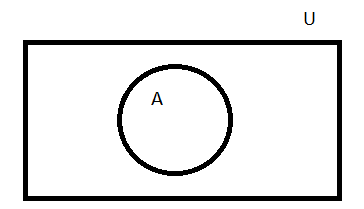
\includegraphics{./img/BasicVenn.png}

Using a Venn diagram, it becomes easy to represent a lot of things in set theory. For example, if $B \subseteq A$, it can be drawn like this

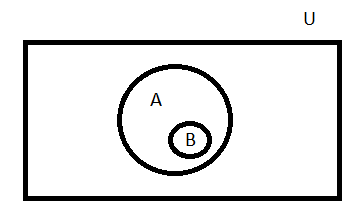
\includegraphics{./img/SubsetVenn.png}

\section*{Set operations}
In the following, the shaded regions in each Venn diagram represents the operation we are talking about.

\begin{itemize}
\item  Union - The union of two sets $A$ and $B$ is defined as the set of elements that are either in $A$ or in $B$ (elements that are in both sets are included!). It is represented as $A \cup B$

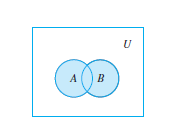
\includegraphics{./img/Union.png}

\item Intersection - this is defined as the set of all elements that are in both $A$ and in $B$. It is represented as $A \cap B$.

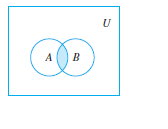
\includegraphics{./img/Intersect.png}

\item Difference - The difference of $B$ minus $A$, denoted $B - A$ refers to the set consisting of elements in $B$ that are not in $A$.

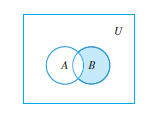
\includegraphics{./img/Difference.png}

\item Complement - the complement of $A$, denoted as $\bar{A}$ is the set of all elements in $U$ that are not in $A$.

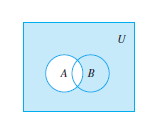
\includegraphics{./img/Complement.png}

\end{itemize}

It is also a good time to get used to writing these in mathematical manner.

\begin{align*}
A \cup B &= \{x \in U | x \in A \text{ or } x \in B\} \\
A \cap B &= \{x \in U | x \in A \text{ and } x \in B \} \\
B - A &= \{x \in B | x \not \in A\} \\
\bar{A} &= \{x \in U | x \not \in A\}
\end{align*}


\section*{Properties}
\begin{itemize}
\item $A \cup B = B \cup A $ - commutative law
\item $A \cap B = B \cap A$ - commutative law
\item $A \cap (B \cap C) = (A \cap B) \cap C$ - associative law
\item $A \cup (B \cup C) = (A \cup B) \cup C$ - associative law
\item $A \cup (B \cap C) = (A \cup B) \cap (A \cup C)$ - distributive law
\item $A \cap (B \cup C) = (A \cap B) \cup (A \cap C)$ - distributive law
\item $A \cap \emptyset = \emptyset$
\item $A \cup U = U$
\item $A \cap U = A$
\item $A \cup \emptyset = A$

\end{itemize}

\subsection*{De-Morgan's laws}
De-Morgan's laws which you might have seen as part of logic, translate very easily into set theory.

\begin{align*}
\overline{(A \cup B)} &= \bar{A} \cap \bar{B} \\
\overline{(A \cap B)} &= \bar{A} \cup \bar{B}
\end{align*}

\subsubsection*{Examples}
Show that $\overline{\bar{A} \cap U} = A$

We simplify this using the properties of sets

\begin{align*}
\overline{\bar{A} \cap U} &= \bar{\bar{A}} \cup \bar{U} & \text{de-morgan's}\\
&= A \cup \bar{U} & \text{complement of a complement is the set itself}\\
&= A \cup \emptyset & \text{complement of the universe = empty!}\\
&= A
\end{align*}

Show that $(A \cap B) \cup \overline{(A \cup \bar{B})} = B$

\begin{align*}
\text{the left side} &= (A \cap B) \cup (\bar{A} \cap B)  & \text{      de-morgan's}\\
&= (A \cup \bar{A}) \cap B & \text{     distributive property}\\
&= U \cap B & \text{  the union of a set and its complement will be the universal set} \\
&= B 
\end{align*}

\section*{Cardinality}
The number of elements in a finite set is called the cardinality of that set.
$A$ is a set, the cardinality is denoted by $|A|$.

What is the cardinality of the set $S = \{\{1\},\{1,2\}\}$?

Be careful, this is a set of sets!  Cardinality is 2 and not 3.

\section*{Power set}

The power set of a set A is the set of all subsets of A and is denoted P(A).

An important thing to remember about the power set of $A$ is that the empty set $\emptyset$ and the set $A$ itself, are both subsets of $A$.

What do you think $|P(A)|$ is?

\pagebreak

\section*{CS application}

Databases - A lot of query syntax involves very basic set theory. 

Made up Examples

There is an retirement agency that is interested in knowing the employees in MS and Apple that are close to retirement. 

Actual SQL syntax would look something like

\begin{verbatim}
SELECT Name, EmployeeId
FROM MSEmployees
WHERE age > 58

UNION

SELECT Name, EmployeeId
FROM AppleEmployees
WHERE age > 58
\end{verbatim}

Tell me what I ate for lunch but did not eat for dinner. Set difference!

\begin{verbatim}
SELECT item FROM Lunch
WHERE consumer = 'Arvind'
EXCEPT
SELECT item FROM Dinner
WHERE consumer = 'Arvind'
\end{verbatim}

\end{document}



